% cascade II /mnt/backup/safe-with-time/torben/safed/y2009/0414
% andor ultra ~/1114  python code for calibration and andor basic for acquisition
\chapter{Read noise characterization of cameras}
\label{sec:ccd-meas}
\begin{summary}
  We describe a method to measure the read noise of a camera and
  compare the performance of three EM-CCDs.
\end{summary}
\section{Introduction}
In order to characterize a camera we captured sequences of images that
contain a light pattern as displayed in \figref{fig:calib-pic}. The
pattern is smooth and non-uniform.
\begin{figure}[!hbt]
  \centering
  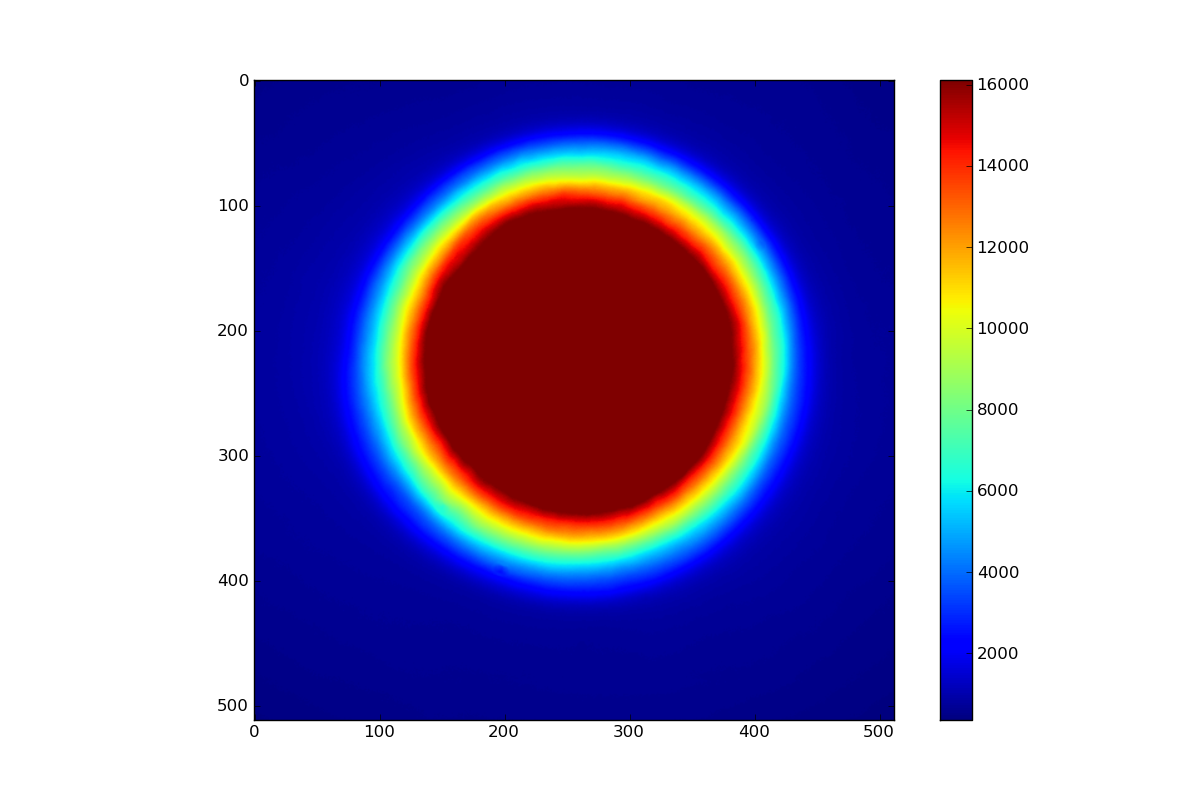
\includegraphics[width=10cm]{calib-pic}
  \caption{Image of a defocused area on a fluorescent plane
    sample. Several such images ($20$) are captured and variance in
    each pixel is plotted against the intensity to find the
    correspondence between reported ADU and detected photoelectrons.}
  \label{fig:calib-pic}
\end{figure}
The images were produced in a fluorescence microscope. The light
source is a DPSS laser with \unit[473]{nm} wavelength. It illuminates
a circular area of the sample, which is a green fluorescent plane. A
FITC filter cube and a $10\times$ objective were used. The sample was
adjusted to be slightly out-of-focus in order to obtain a smooth
intensity gradient in the image.

The light source is stable and the relative standard deviation of the
illumination intensity is typically $<0.2\%$ for the calibration
time. 

A sequence (20) of such images can be used to determine the mapping
between analog-to-digital units (ADU)
\nomenclature{ADU}{analog-to-digital unit} and the number of detected
photoelectrons. This method is based on the known relation between the
mean number of Poisson distributed photons and its variance.

For the calibration a 2D histogram of the per pixel
variance image and the per pixel mean of the image stack is
plotted. Then the slope of the resulting point cloud is determined.

\section{Calibration of an Andor IXon3 camera}

\begin{figure}
  \centering
  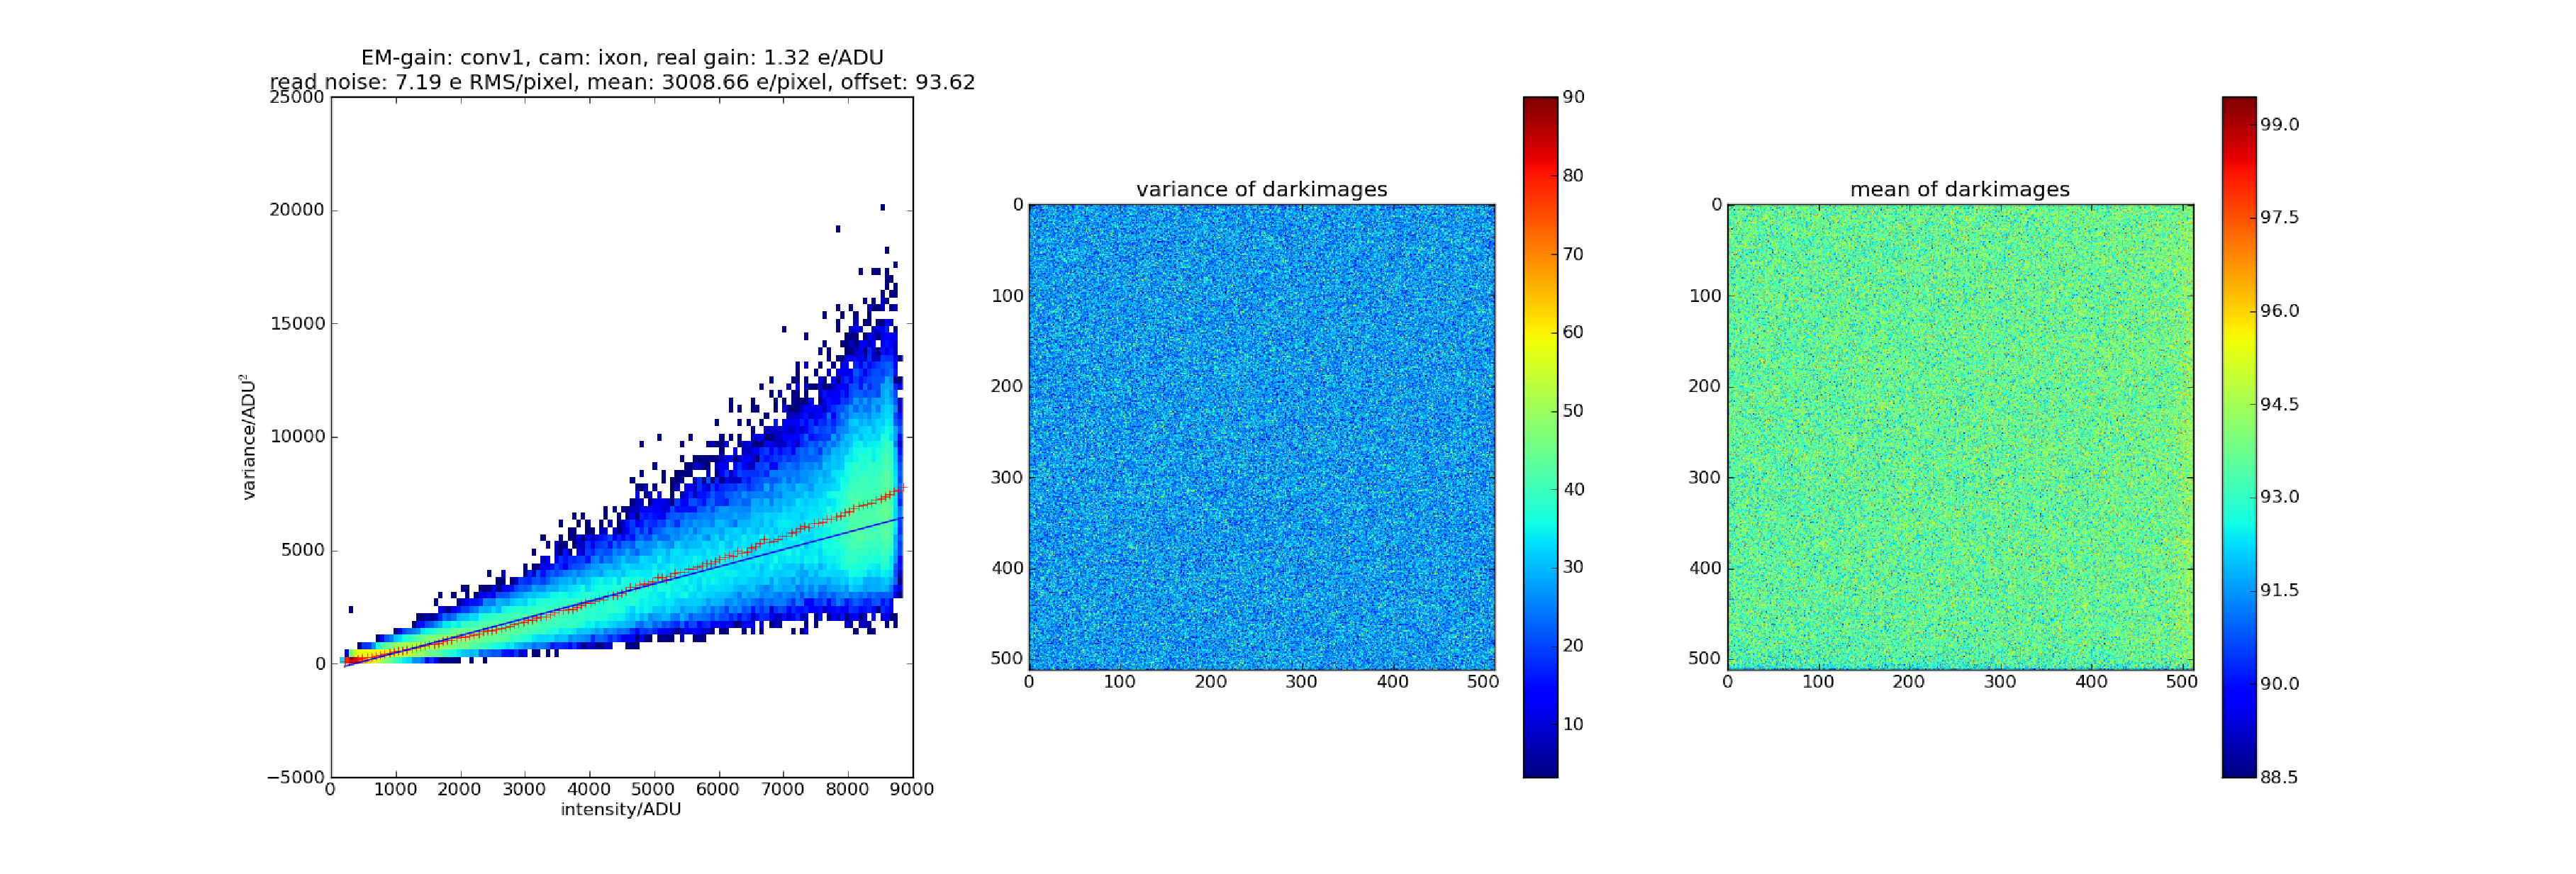
\includegraphics[width=14cm]{../app_cam/ixon_conv1}
  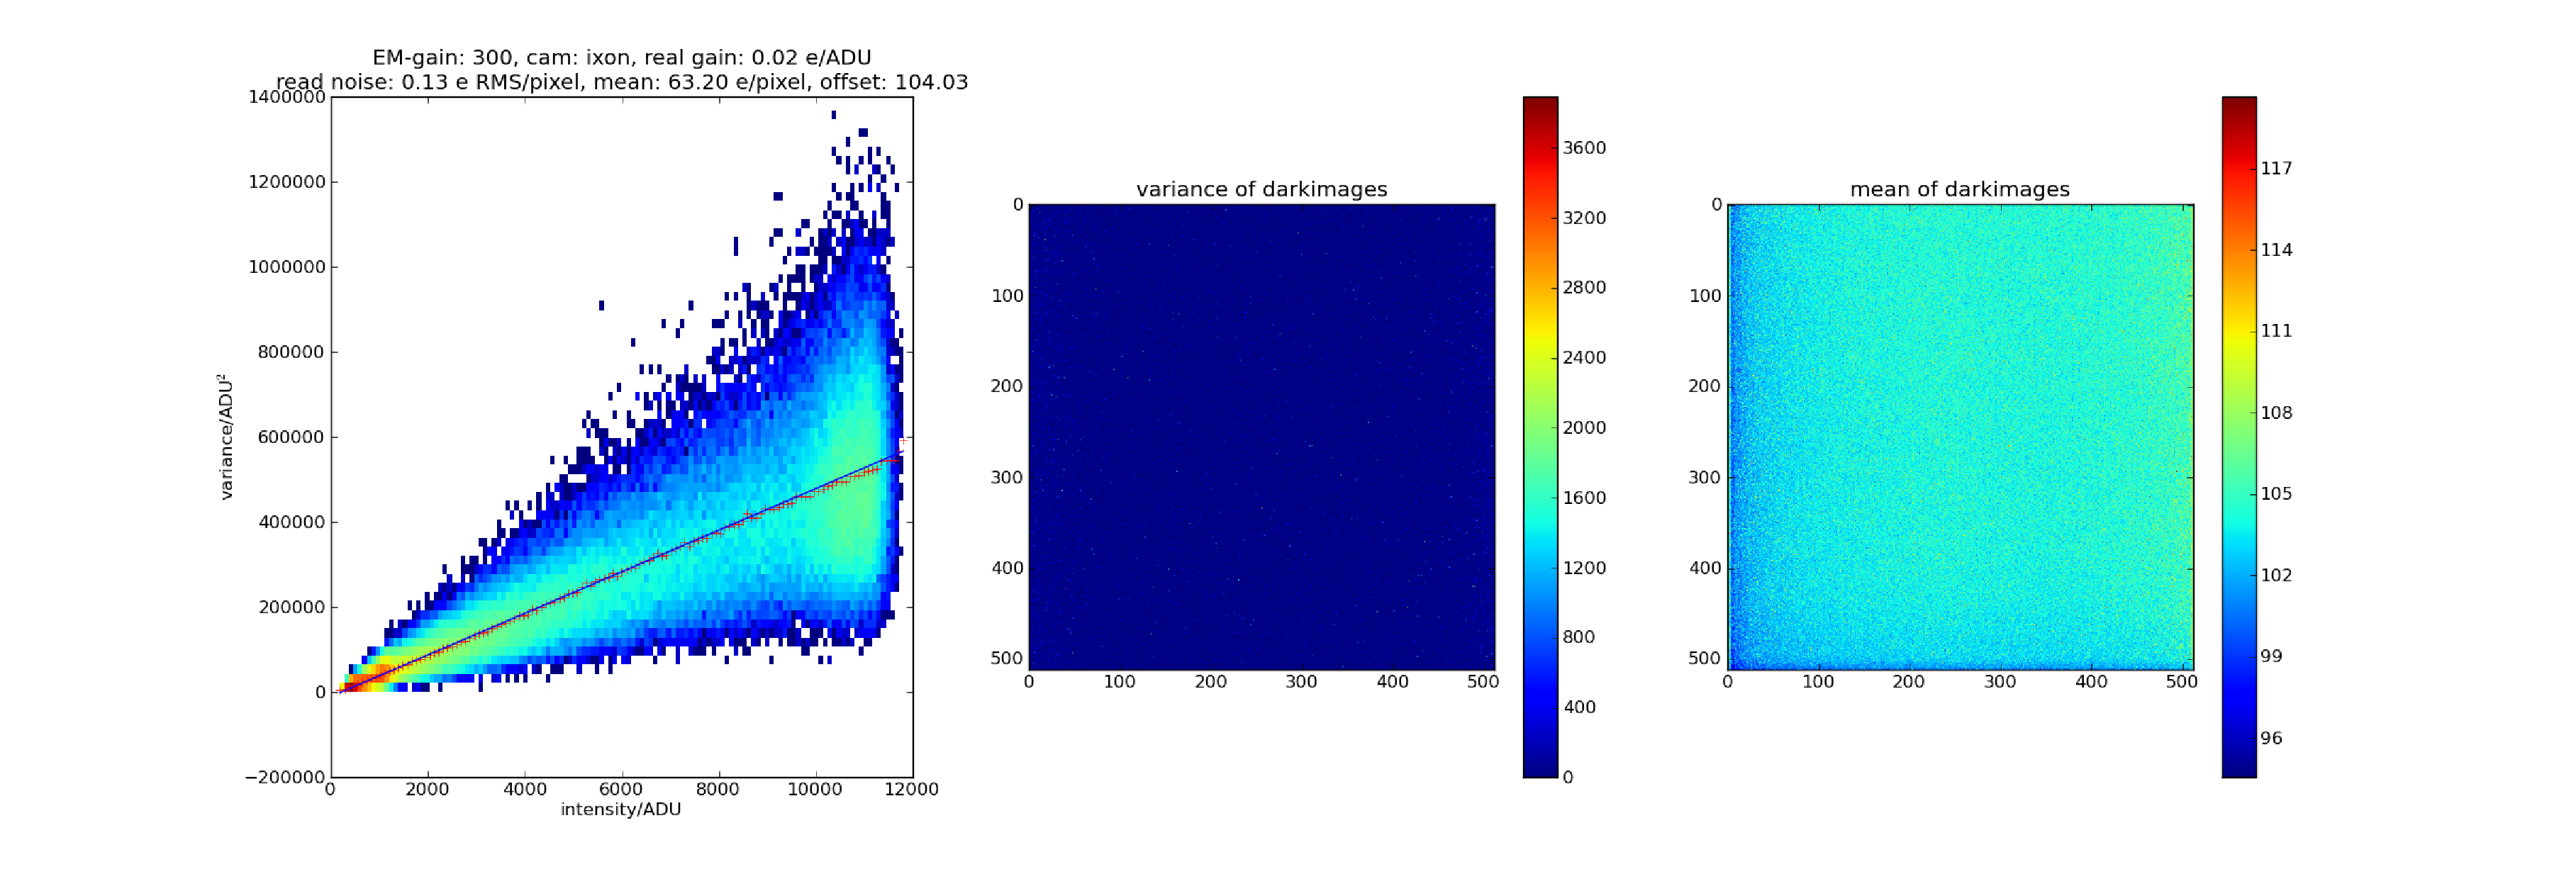
\includegraphics[width=14cm]{../app_cam/ixon_300}
  \caption{{\bf top:} Conventional readout of an Andor IXon3
    camera. {\bf bottom:} readout with an EM-gain setting of 300 on
    the same camera with identical sample. {\bf left:} 2D histogram of
    per pixel variances against binned intensities. {\bf middle:}
    variance of 20 dark images. {\bf right:} mean of 20 dark images.}
  \label{fig:ixon}
\end{figure}
  
The top left diagram of \figref{fig:ixon} contains such a 2D
histogram. It was obtained by conventional readout at \unit[3]{MHz} of
our Andor IXon3 camera (head: DU-897D-CS0-\#BV). The variances are
collected in 64 intensity bins and their averages are plotted as red
crosses. The blue line is the result of a linear fit to the first
$60\%$ of the red crosses. Its slope gives the real gain of the camera
that can be used to convert ADU into photoelectrons (here
\unit[1.32]{$e/$ADU}).

The following figures show corresponding measurements using the EM
readout mode with varying EM-gain. It is followed by one last
measurement with conventional readout to verify, that the fluorophores
didn't bleach too much during the experiment.

The camera was cooled to \unit[$-75$]{$\,^{\circ}{\rm C}$}. In order
to prevent overexposure of the sensor a preliminary image with a short
integration time of \unit[10]{ms} was acquired. Then, using this
image, the integration time was for the experiment was set such that a
maximum of \unit[10000]{ADU} would occur (in the function
\textsf{$\sim$GetSaturationExposure}). An internal shutter in the camera
was closed (\textsf{SetShutter}) to obtain the dark images. The process
was automated using an Andor Solis Basic program which is listed
below.


The square root of the mean of the variance of the dark images was
converted into a read noise in electrons per pixel using the real
gain.

Table~\ref{tab:ixon-table} summarizes the calibration results. The
average of the dark images (in ADU) is given in the column
\textsf{offset}. The read noise in conventional mode is approximately
8 electrons per pixel rms. The column \textsf{mean'} contains the
average number of photoelectrons per pixel in the illuminated image
normalized by the integration time. The rows \textsf{conv1} and
\textsf{conv2} with conventional readout (without EM-gain) contain
approximately the same number. This proves that no significant
bleaching occurred during the experiment.

The EM-gain process introduces multiplicative noise in the signal. Its
effect on the photoelectron statistics is the same as lowering the
quantum efficiency of the sensor. Dividing values of the column
\textsf{ mean'} from EM readouts by the same value from the
conventional readout gives the \emph{excess noise factor}\todo{get
  this right: should be $\sqrt{2}$}. Its value is smaller than one and
describes the apparent reduction of the quantum efficiency.


% Due to a bug in the capturing process the images in the second row
% (for EM-gain 40) was overexposed and the data shouldn't be used.  Also
% the last experiment \textsf{conv2} with conventional readout reports
% a larger gain of \unit[1.6]{e/ADU} than the first experiment
% \textsf{conv1} with gain \unit[1.3]{e/ADU}. Later we learned that one
% should allow several seconds of settling time, when changing the
% EM-gain voltage. This might explain the difference in gains, even
% though one would think that the conventional readout should be
% decoupled.


\begin{table}[!htbp]
  \centering
  \begin{tabular}{|l|l|l|l|l|l|l|l|}
\hline
\textsf{Ixon3} & \textsf{gain} & \textsf{noise} & \textsf{mean} & \textsf{offset} & \textsf{exp time} & \textsf{mean'} & \textsf{excess} \\
 & [e/ADU] & [e/px] & [e/px] & [ADU] & [s] & [e/(px s)] & \\
\hline
conv1 & 1.3165 & 7.189 & 3008.66 & 93.62 & 0.2016 & 14923 & 0.981 \\
\hline
50 & 0.1160 & 0.486 & 260.05 & 103.23 & 0.0289 & 8995 & 0.591 \\
\hline
60 & 0.0984 & 0.406 & 225.46 & 103.26 & 0.0249 & 9054 & 0.595 \\
\hline
70 & 0.0841 & 0.349 & 190.52 & 103.49 & 0.0212 & 8983 & 0.591 \\
\hline
80 & 0.0729 & 0.305 & 165.24 & 103.17 & 0.0186 & 8907 & 0.586 \\
\hline
90 & 0.0680 & 0.288 & 150.54 & 103.34 & 0.0161 & 9368 & 0.616 \\
\hline
100 & 0.0611 & 0.262 & 128.47 & 103.35 & 0.0136 & 9427 & 0.620 \\
\hline
110 & 0.0550 & 0.241 & 121.11 & 103.73 & 0.0129 & 9409 & 0.619 \\
\hline
120 & 0.0510 & 0.228 & 113.71 & 103.50 & 0.0120 & 9498 & 0.624 \\
\hline
130 & 0.0465 & 0.211 & 106.66 & 103.63 & 0.0112 & 9541 & 0.627 \\
\hline
140 & 0.0433 & 0.201 & 96.95 & 103.77 & 0.0101 & 9564 & 0.629 \\
\hline
150 & 0.0405 & 0.192 & 89.68 & 103.79 & 0.0093 & 9671 & 0.636 \\
\hline
160 & 0.0380 & 0.183 & 87.24 & 103.87 & 0.0090 & 9656 & 0.635 \\
\hline
170 & 0.0359 & 0.175 & 81.56 & 104.17 & 0.0084 & 9739 & 0.640 \\
\hline
180 & 0.0339 & 0.169 & 79.80 & 104.00 & 0.0081 & 9863 & 0.648 \\
\hline
190 & 0.0321 & 0.163 & 74.00 & 104.26 & 0.0075 & 9806 & 0.645 \\
\hline
200 & 0.0305 & 0.158 & 72.57 & 104.03 & 0.0073 & 9878 & 0.649 \\
\hline
210 & 0.0292 & 0.155 & 69.44 & 104.22 & 0.0070 & 9944 & 0.654 \\
\hline
220 & 0.0280 & 0.150 & 67.69 & 104.08 & 0.0068 & 9971 & 0.656 \\
\hline
230 & 0.0268 & 0.147 & 65.63 & 104.03 & 0.0065 & 10057 & 0.661 \\
\hline
240 & 0.0257 & 0.188 & 63.90 & 104.05 & 0.0063 & 10131 & 0.666 \\
\hline
250 & 0.0244 & 0.140 & 62.52 & 104.15 & 0.0062 & 10026 & 0.659 \\
\hline
260 & 0.0237 & 0.137 & 62.86 & 104.18 & 0.0062 & 10078 & 0.663 \\
\hline
270 & 0.0229 & 0.135 & 63.17 & 103.94 & 0.0062 & 10130 & 0.666 \\
\hline
280 & 0.0221 & 0.133 & 63.64 & 104.21 & 0.0062 & 10204 & 0.671 \\
\hline
290 & 0.0214 & 0.130 & 63.38 & 104.15 & 0.0062 & 10162 & 0.668 \\
\hline
300 & 0.0205 & 0.128 & 63.20 & 104.03 & 0.0062 & 10133 & 0.666 \\
\hline
conv2 & 1.5953 & 8.768 & 8198.86 & 93.30 & 0.5291 & 15496 & 1.019 \\
\hline
\end{tabular}
%  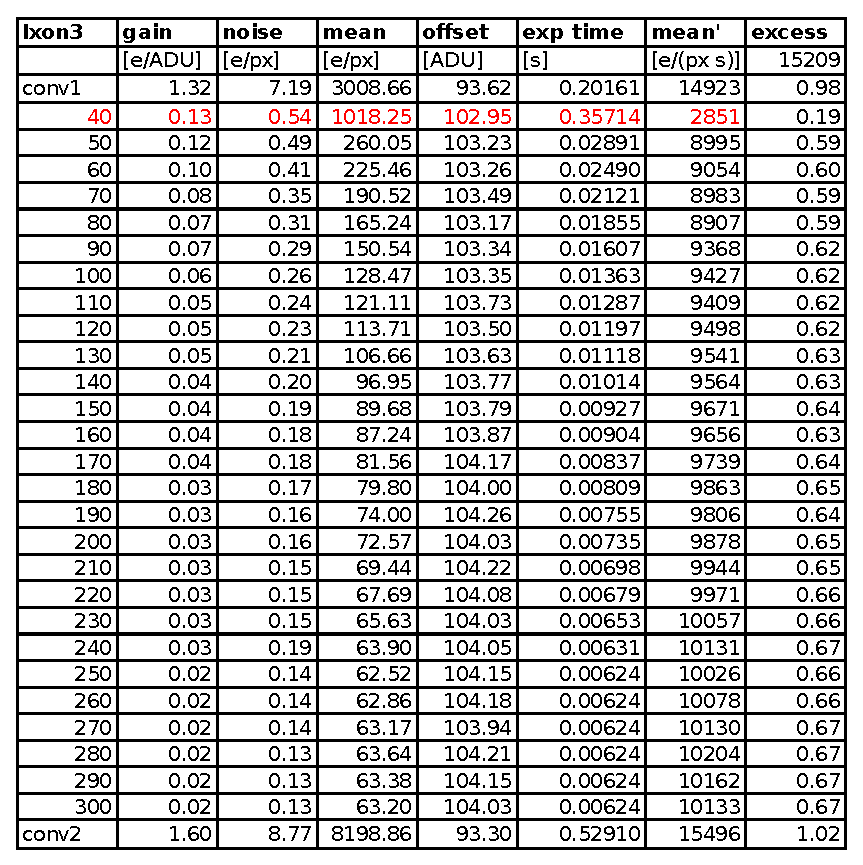
\includegraphics[width=12cm]{../app_cam/ixon3}
  \caption{Comparison of read noise for different EM-gain settings
    (first column) of the Andor IXon3. The value $\textsf{mean}'$
    estimates the number of photoelectrons the detector would have
    seen with \unit[1]{s} integration time and is used to calculate
    the excess noise factor in the last column. In EM-mode the fastest
    readout speed was used \unit[10]{MHz} with vertical shift speed of
    \unit[1.7]{$\mu$s}.}
  \label{tab:ixon-table}
\end{table}


\subsection{Andor Basic code listing for automatic image acquisition}
{\small
\begin{verbatim}
function ~GetSaturatingExposure()
        SetKineticNumber(1)
        exp=.01
        SetExposureTime(exp)
        run()
        m=maximum(#0,1,512)
        GetSaturatingExposure=exp*10000/(m-100)
        CloseWindow(#0)
return
name$ = "C:\Users\work\Desktop\martin\20111111\scan-em3\ixon_"
print("start")

SetOutputAmp(1)
print("conv_start")
exp= ~GetSaturatingExposure()
print(exp)
SetExposureTime(exp)
SetKineticNumber(20)
SetShutter(0,1)
run()
save(#0,name$ + "conv1_dark.sif")
ExportTiff(#0, name$ + "conv1_dark.tif", 1, 1, 0, 0)
CloseWindow(#0)
CloseWindow(#1)
        
SetShutter(1,1)
run()
save(#0,name$ + "conv1_bright.sif")
ExportTiff(#0, name$ + "conv1 _bright.tif", 1, 1, 0, 0)
CloseWindow(#0)
CloseWindow(#1)

SetOutputAmp(0)
SetShutter(1,1)
for i = 40 to 300 step 10
        SetGain(i)
        exp=~GetSaturatingExposure()
        print(exp)
        SetExposureTime(exp)
        SetKineticNumber(20)
        SetShutter(0,1)
        run()
        save(#0,name$ + str$(i) + "_dark.sif")
        ExportTiff(#0, name$ + str$(i) + "_dark.tif", 1, 1, 0, 0)
        CloseWindow(#0)
        CloseWindow(#1)
        SetShutter(1,1)
        run()
        save(#0,name$ + str$(i) + "_bright.sif")
        ExportTiff(#0, name$ + str$(i) + "_bright.tif", 1, 1, 0, 0)
        CloseWindow(#0)
        CloseWindow(#1)
next

SetOutputAmp(1)
print("conv_end")
exp= ~GetSaturatingExposure()
print(exp)
SetExposureTime(exp)
SetKineticNumber(20)
SetShutter(0,1)
run()
save(#0,name$ + "conv2_dark.sif")
ExportTiff(#0, name$ + "conv2_dark.tif", 1, 1, 0, 0)
CloseWindow(#0)
CloseWindow(#1)
        
SetShutter(1,1)
run()
save(#0,name$ + "conv2_bright.sif")
ExportTiff(#0, name$ + "conv2 _bright.tif", 1, 1, 0, 0)
CloseWindow(#0)
CloseWindow(#1)
\end{verbatim}
}

\subsection{Python code listing for the read noise evaluation}
{\small
\begin{verbatim}
#!/usr/bin/env python
# ./ti.py /media/backup/andor-ultra-ixon/martin/20111111/scan-em3/ ultra 2700
import sys
import os

import matplotlib
matplotlib.use('Agg')

from pylab import *
from libtiff import TIFFfile, TIFFimage
from scipy import stats

seterr(divide='ignore')

folder = sys.argv[1]
cam = sys.argv[2]
gain = sys.argv[3]

def readpics(gain,cam='ixon_',isdark=False):
    print 'loading ', os.path.join(folder,cam) + '_' + gain + '_bright.tif'
    fg=TIFFfile(os.path.join(folder,cam) + '_' + gain + '_bright.tif')
    bright,bright_names=fg.get_samples()
    bg=TIFFfile(os.path.join(folder,cam) + '_' + gain + '_dark.tif')    
    dark,dark_names=bg.get_samples()
    return (bright[0],dark[0])

(f,b) = readpics(gain=gain,cam=cam)

bg=mean(b,axis=0)
v=var(f,axis=0)
i=mean(f,axis=0)

ny,nx=64,128
H,y,x=histogram2d(v.flatten(),i.flatten(),bins=[ny,nx],
                  range=[[0,v.max()],[0,i.max()]])
extent = [x[0], x[-1], y[0], y[-1]] 
acc=zeros(x.shape,dtype=float64)
accn=zeros(x.shape,dtype=int64)
s=nx/i.max()
for ii,vv in nditer([i,v]):
    p=round(ii*s)
    acc[p]+=vv
    accn[p]+=1   

fig=figure(figsize=(24, 8),dpi=300)
hold(False)
title('bal')
subplot(1,3,1)
imshow(log(H), extent=extent,
           aspect='auto', interpolation='none',origin='lower')
hold(True)
ax=x[nonzero(accn)]
ay=acc/accn
ay=ay[nonzero(accn)]
l=round(.6*len(ax))
bx=ax[0:l]
by=ay[0:l]
plot(ax,ay,'r+')
slope,intercept,rval,pval,stderr=stats.linregress(bx,by)
plot(ax,polyval([slope,intercept],ax))
xlabel('intensity/ADU')
ylabel(r'variance/ADU$^2$')
real_gain=1/slope # unit electrons/ADU
read_noise=sqrt(var(b))*real_gain # electrons RMS per pixel
mean_elecs=(mean(f)-mean(b))*real_gain # photoelectrons electrons per pixel
print gain,cam,real_gain,read_noise,mean_elecs,mean(b),rval,pval,stderr
tit='EM-gain: %s, cam: %s, real gain: %.2f e/ADU\n
read noise: %.2f e RMS/pixel, mean: %.2f e/pixel, offset: %.2f'
% (gain,cam,real_gain,read_noise,mean_elecs,mean(b))
title(tit)
subplot(1,3,2)
imshow(var(b,axis=0))
title('variance of darkimages')
colorbar()
subplot(1,3,3)
imshow(mean(b,axis=0))
title('mean of darkimages')
colorbar()
show()
fig.savefig(cam+'_'+gain+'.png')
\end{verbatim}
}

\section{Comparison with other cameras}
The values of the EM-gain parameter in the camera software are in
general not easily related to the actual amplification factor
happening in the EM registers of the chip (changes with temperature
and ages during the sensors life). 

In order to compare different EM-CCD cameras we first convert the
EM-gain parameter setting into the real EM-gain. For this, we divide
the real gain (\textsf{gain}) of the respective EM readout to the real
gain of the conventional readout.

\figref{fig:old-cams} shows some calibrations on older cameras (Andor
IXon2 (head: DU-897E-CS0-\#BV, sensor: E2V Tech CCD97 $512\times512$,
pixel pitch \unit[16]{$\mu$m}, cooled to $-70{}^\circ\textrm{C}$) and
Photometrics Cascade~II (sensor: e2v CCD97, $512\times512$, pixel
pitch \unit[16]{$\mu$m}, cooled to $-70{}^\circ\textrm{C}$) which were
performed using the DIPimage function \textsf{cal-readnoise}
\citep{Lidke2005a}.  The real EM-gain of the Andor IXon2 is
$0.67/0.062=10.8$ and it has \unit[0.46]{e\ rms/pixel} readnoise. The
real EM-gain of the Cascade~II is $1.6/0.14=11.4$ with \unit[1.13]{e\
  rms/pixel} read noise. Approximately the same real gain is obtained
with the IXon3 at EM-gain 50: $1.32/0.12=11.0$ with a read noise of
\unit[0.49]{e\ rms/pixel}. So the two Andor cameras show the same
performance.

\begin{figure}
  \centering
  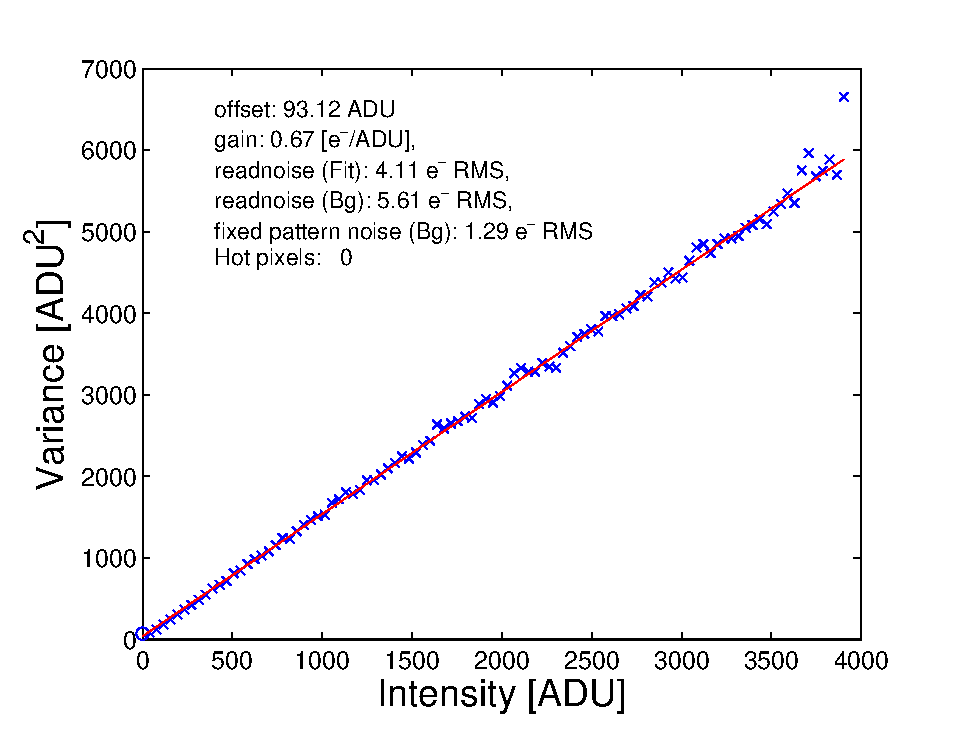
\includegraphics[width=7cm]{../app_cam/andor_normal_preamp5_exp30}
  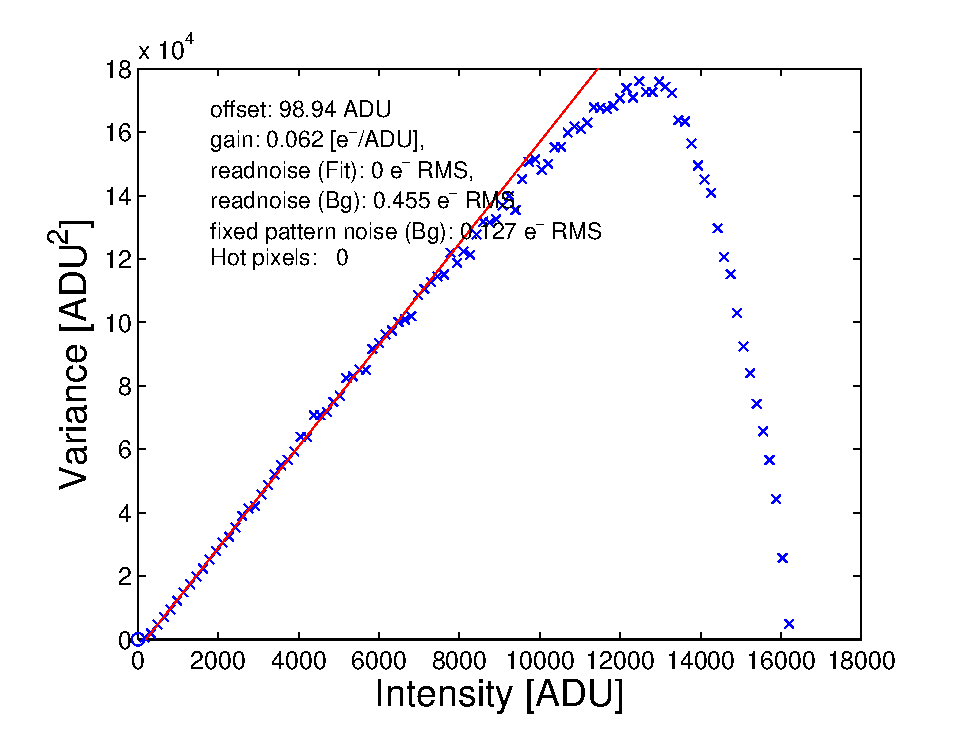
\includegraphics[width=7cm]{../app_cam/andor_emgain100_preamp5_exp30}
  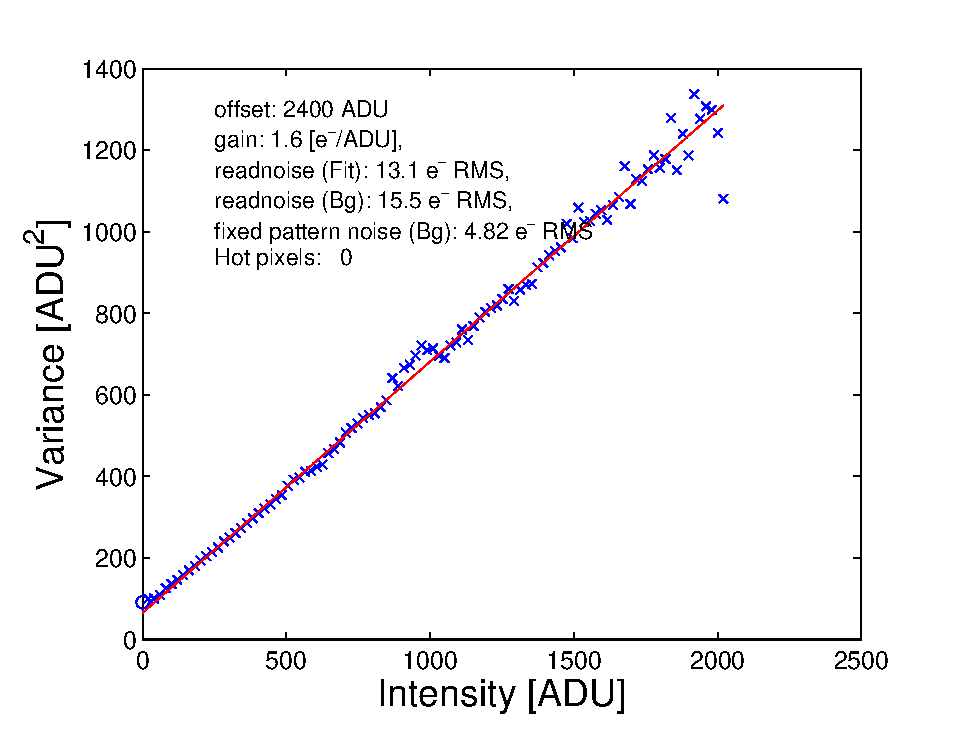
\includegraphics[width=7cm]{../app_cam/cascade_exp400ms_normal}
  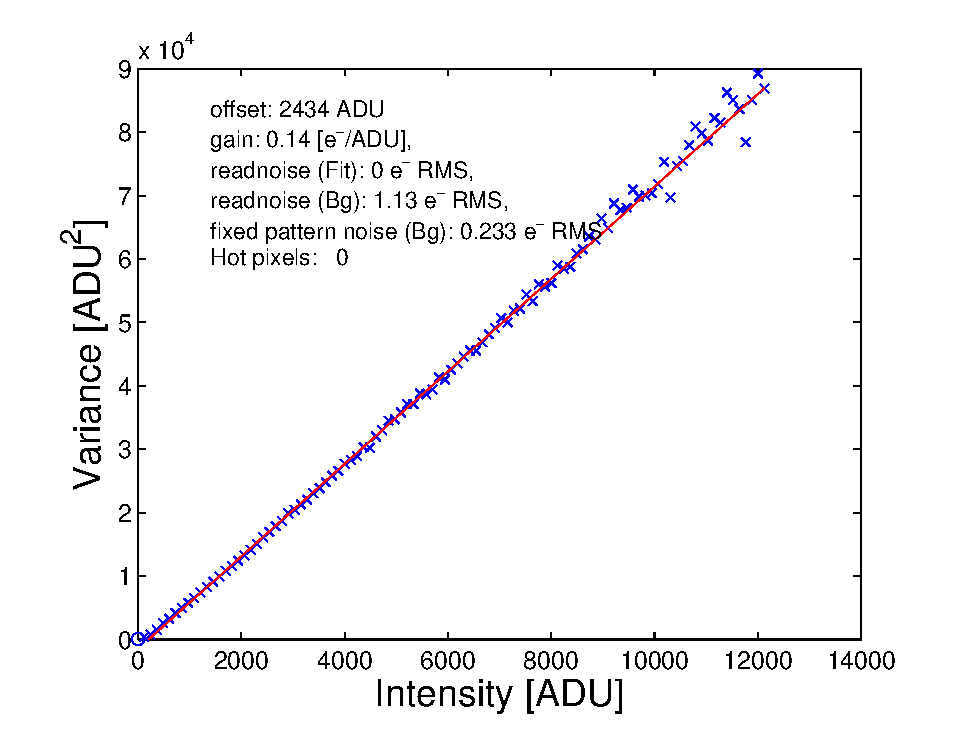
\includegraphics[width=7cm]{../app_cam/cascade_exp400ms_gain3000}
  % \includegraphics[width=7cm]{../app_cam/cascade_normal_preamp3_exp30}
  \caption{{\bf top:} Andor IXon2 {\bf left:} Normal readout with
    preamp 5. {\bf top right:} EM-gain 100 preamp 5. {\bf bottom:}
    Cascade II {\bf left:} Normal readout
    $\textsf{mean}=\unit[254.82]{e/pixel}$. {\bf right:} EM-gain 3000,
    $\textsf{mean}=\unit[122.08]{e/pixel}$, therefore the excess noise
    factor is 0.48.}
  \label{fig:old-cams}
\end{figure}

% sushi 20090414 maybe check for readout speed of cascade II and the
% excess noise factor of the andor

% check in lab book for exact specs of andor ixon2

